\documentclass{article}
\usepackage{nips10submit_e,times}
%\documentstyle[nips07submit_09,times]{article}
\usepackage[square,numbers]{natbib}
\usepackage{amsmath, epsfig}
\usepackage{amsfonts}
\usepackage{subfigure}
\usepackage{graphicx}
\usepackage{amsfonts}
\usepackage{algorithm}
\usepackage{algorithmic}
\usepackage{easybmat}
\usepackage{footmisc}
\usepackage{lscape}
\renewcommand\algorithmiccomment[1]{// \textit{#1}}
%
\newcommand{\ignore}[1]{}
\newcommand{\comment}[1]{}
\DeclareMathOperator*{\argmax}{arg\,max}

\title{Hierarchically Supervised Latent Dirichlet Allocation}
%Supervised Topic Modeling in Clinical Text}

\author{
Adler Perotte\hspace{1cm} Nicholas Bartlett \hspace{1cm} Noemie Elhadad \hspace{1cm} Frank Wood\\
Columbia University, New York, NY 10027, USA \\
\texttt{\{ajp9009@dbmi,bartlett@stat,noemie@dbmi,fwood@stat\}.columbia.edu}
%\texttt{pfau@neurotheory.columbia.edu} 
%\texttt{\{bartlett,fwood\}@stat.columbia.edu} 
}



% The \author macro works with any number of authors. There are two commands
% used to separate the names and addresses of multiple authors: \And and \AND.
%
% Using \And between authors leaves it to \LaTeX{} to determine where to break
% the lines. Using \AND forces a linebreak at that point. So, if \LaTeX{}
% puts 3 of 4 authors names on the first line, and the last on the second
% line, try using \AND instead of \And before the third author name.

\newcommand{\fix}{\marginpar{FIX}}
\newcommand{\new}{\marginpar{NEW}}
\newcommand{\X}{\mathcal{X}}


\nipsfinalcopy

\begin{document}

\maketitle

\begin{abstract}


We introduce hierarchically supervised latent Dirichlet allocation (HSLDA), a
model for hierarchically and multiply labeled bag-of-word data.  Examples of
such data include web pages and their placement in directories, product
descriptions and associated categories from product hierarchies, and free-text
clinical records and their assigned diagnosis codes. Out-of-sample label
prediction is the primary goal of this work, but improved lower-dimensional
representations of the bag-of-word data are also of interest.
%% We demonstrate HSLDA on large-scale data from clinical document labeling and
%% retail product categorization tasks. We show that leveraging the structure from
%% hierarchical labels improves out-of-sample label prediction substantially when
%% compared to models that do not. 

Our work operates within the framework of topic modeling. Our approach learns
topic models of the underlying data and labeling strategies in a joint model,
while leveraging the hierarchical structure of the labels. For the sake of
simplicity, we focus on is-a hierarchies, but the model can be
applied to other structured label spaces. Our work extends supervised latent Dirichlet
allocation (sLDA)~\cite{BleiMcAuliffe2008} to take advantage of hierarchical
supervision and proposes an efficient way to incorporate such information into the model. 
We hypothesize that the context of labels within
the hierarchy provides valuable information about labeling. Other models, such as LabeledLDA~\citep{Ramage2009}, incorporate LDA and supervision; however, none of these models leverage dependency structure in the label space.

We demonstrate our model on large, real-world datasets in the clinical and web
retail domains. We observe that hierarchical information is valuable when
incorporated into the learning and improves our primary goal of multi-label
classification. Our results show that a joint, hierarchical model outperforms a
classification with unstructured labels as well as a disjoint model, where the
topic model and the hierarchical classification are inferred
independently of each other. 

HSLDA is a model for hierarchically, multiply-labeled, bag-of-word data.  We
will refer to individual groups of bag-of-word data as documents.  Let $w_{n,d}
\in \Sigma$ be the $n$th observation in the $d$th document.  Let $\mathbf{w}_d
= \{w_{1,d},\ldots,w_{1,N_d}\}$ be the  set of $N_d$ observations in document
$d$.  Let there be $D$ such documents and let the size of the vocabulary be
$V=|\Sigma|$.  Let the set of labels be $\mathcal{L}=\left\{
  l_{1},l_{2},\ldots,l_{\left|\mathcal{L}\right|}\right\} $. Each label
$l \in \mathcal{L}$, except root, has a parent $\mathrm{pa}(l) \in \mathcal{L}$
also in the set of labels. 
 We will for exposition purposes assume that this label set has hard ``is-a''
 parent-child constraints, although this assumption can be
 relaxed at the cost of more computationally complex inference.  Such a label hierarchy forms a multiply rooted tree.  Without loss of generality we will consider a tree with a single root $r\in\mathcal{L}$.  Each document has a variable $y_{l,d} \in \{-1,1\}$ for every label which indicates whether the label is applied to document $d$ or not.   In most cases $y_{i,d}$ will be unobserved, in some cases we will be able to fix its value because of  constraints on the label hierarchy, and in the relatively minor remainder its value will be observed.  In the applications we consider, only positive label applications are observed.  


%In HSLDA, the bag-of-word document data is modeled using the LDA
%mixed-membership mixture model with global topic estimation.
In HSLDA, documents are modeled using the LDA mixed-membership mixture model
with global topic estimation. Label responses are generated using a conditional
hierarchy of probit regressors\cite{gelmanbda04}. The HSLDA graphical model is given in
Figure~\ref{fig:graphical_model}. In the model, $K$ is the number of LDA
``topics'' (distributions over the elements of $\Sigma$), $\boldsymbol\phi_k$
is a distribution over ``words,'' $\boldsymbol\theta_d$ is a document-specific
distribution over topics, and $\boldsymbol\beta$ is a global distribution over
topics.
%% , Dir$_{K}(\cdot)$ is a $K$-dimensional Dirichlet distribution,
%% $\mathcal{N}_{K}(\cdot)$ is the $K$-dimensional Normal distribution,
%% $\mathbf{I}_{K}$ is the $K$ dimensional identity matrix,  $\mathbf{1}_d$ is the
%% $d$-dimensional vector of all ones, and $\mathbb{I}(\cdot)$ is an indicator
%% function that takes the value $1$ if its argument is true and $0$ otherwise. 

\begin{figure}[t]
%tbp] %  figure placement: here, top, bottom, or page
 \centering 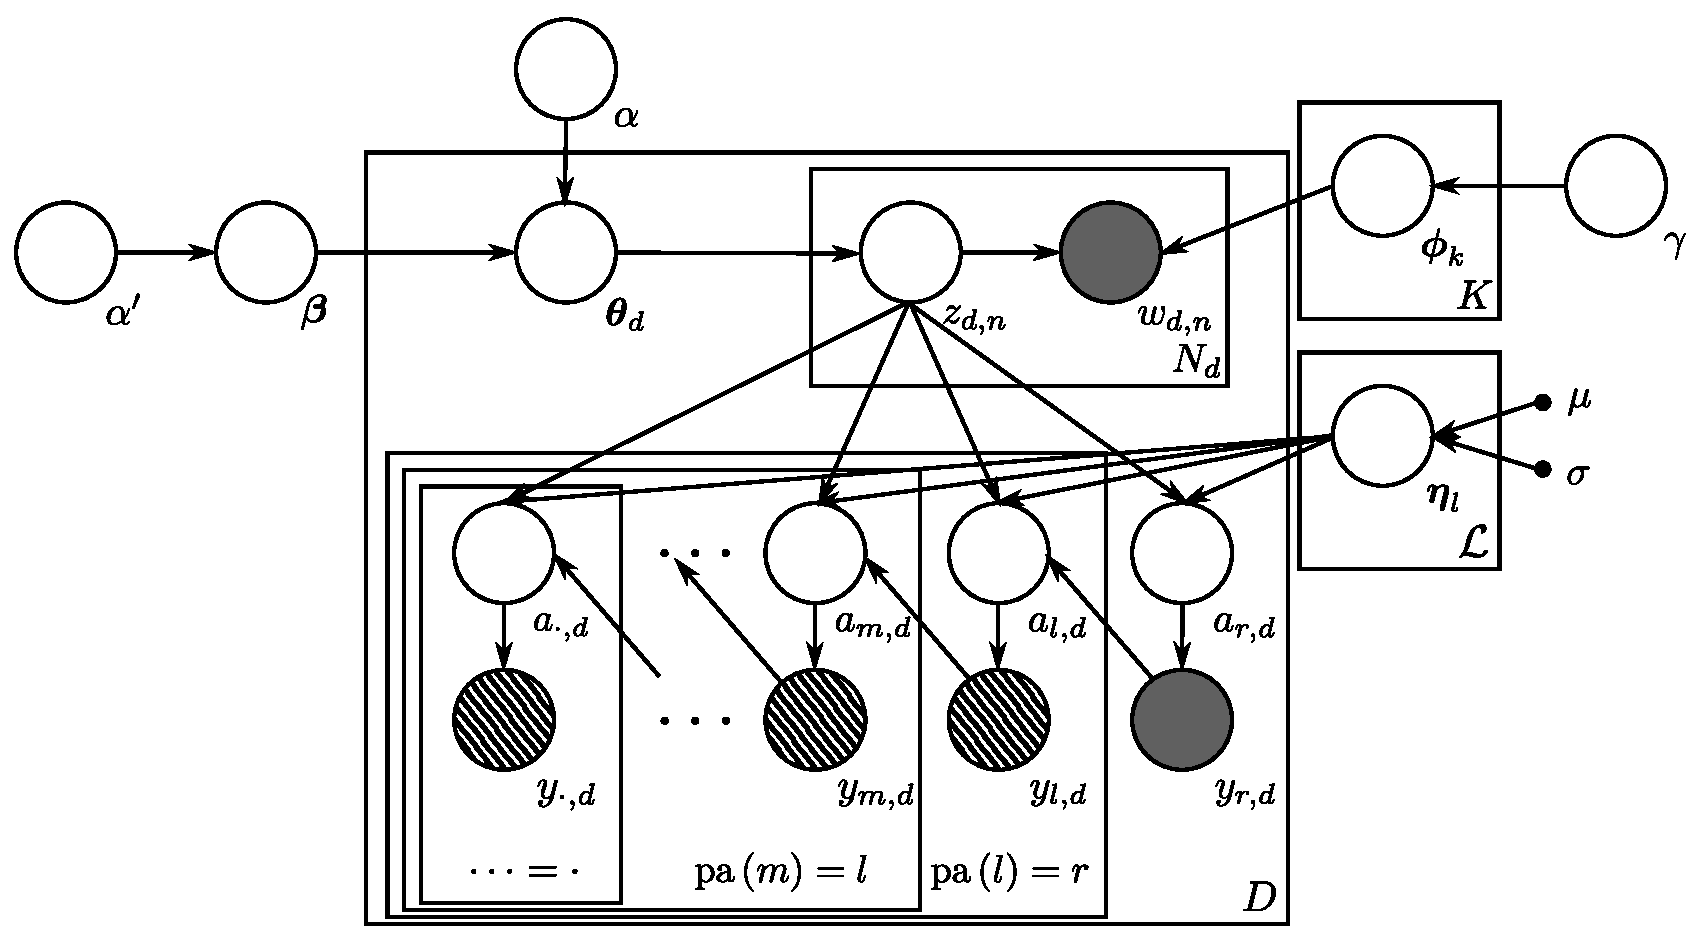
\includegraphics[scale=0.25]{Graphical_Model-final} \caption{HSLDA graphical model}


\label{fig:graphical_model} 
\end{figure}


Posterior inference in HSLDA was performed using Gibbs sampling and Markov chain Monte Carlo.  Note that, like in collapsed Gibbs samplers for LDA \cite{Griffiths04}, we have analytically marginalized out the parameters $\boldsymbol{\phi}_{1:K}$
and $\boldsymbol{\theta}_{1:D}$. HSLDA also employs a hierarchical Dirichlet prior over topic assignments (i.e.,~$\boldsymbol\beta$ is estimated from data rather than assumed to be symmetric).  This has been shown to improve the quality and stability of inferred topics \citep{WallachMiMc2009}. The hyperparameters $\alpha$, $\alpha^{\prime}$, and $\gamma$ are
%given broad ${\rm Gamma}(1,1000)$ prior distributions and 
sampled
using Metropolis-Hastings. 


We applied HSLDA to data from two domains: predicting medical
diagnosis codes from hospital discharge summaries and predicting product
categories from Amazon.com product descriptions. The clinical dataset consists
of 6,000 clinical notes along with associated billing codes that are used
to document conditions that a particular patient was treated for. These billing
codes (7298 distinct codes in our dataset) are organized in an is-a hierarchy. The retail dataset
consists of product descriptions for DVDs from the Amazon.com product catalog. This data
was partially obtained from the Stanford Network Analysis Platform (SNAP) dataset~\citep{SNAP}. The comparison models included sLDA with independent
regressors (hierarchical constraints on labels ignored) and HSLDA fit by first
performing LDA then fitting tree-conditional regressions. The number of topics for all models was set to 50, the prior distributions of
$p\left(\alpha\right)$, $p\left(\alpha^{\prime}\right)$, and
$p\left(\gamma\right)$ were gamma distributed with a shape parameter of 1 and a
scale parameters of 1000. 

\begin{figure}[h]
\begin{center}
%\subfloat[][\label{fig:1a}]{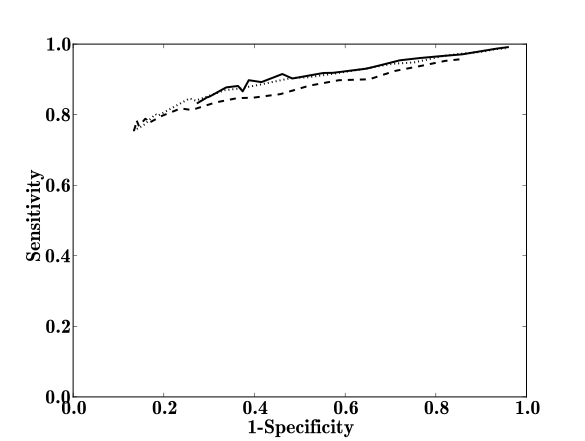
\includegraphics[width=.49\textwidth]{figs/amazon_pred_varying_mu}}
\subfigure[][]{\label{fig:1a}\includegraphics[width=.3\textwidth]{figs/clin_pred_varying_mu}}
%\subfloat[][\label{fig:1c}]{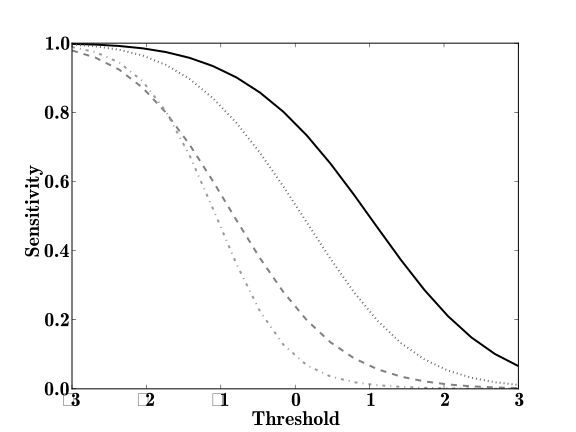
\includegraphics[width=.49\textwidth]{figs/sens_comparison_leafs}}
\subfigure[][]{\label{fig:1b}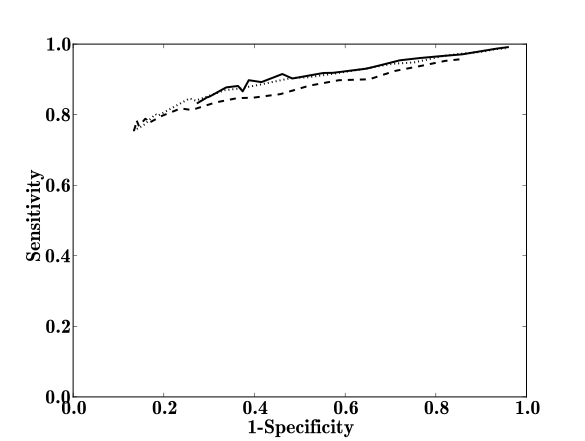
\includegraphics[width=.3\textwidth]{figs/amazon_pred_varying_mu}}
\subfigure[][]{\label{fig:clinical_roc}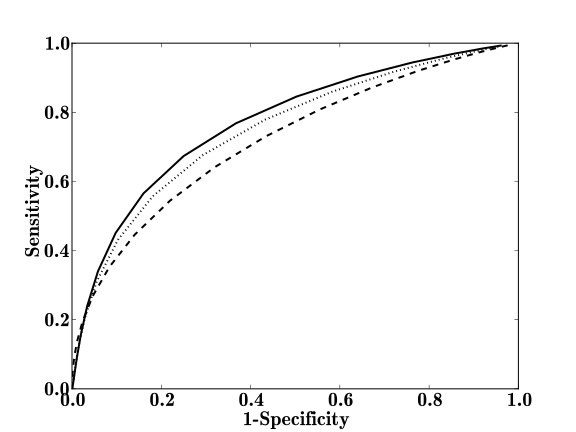
\includegraphics[width=0.3\textwidth]{figs/ROC_comparison_leafs}}
\caption{ROC curves for out-of-sample ICD-9 code prediction from patient free-text discharge records 
(\subref{fig:1a},\subref{fig:clinical_roc}). ROC curve for out-of-sample Amazon product category predictions from 
product free-text descriptions \subref{fig:1b}. Figures \subref{fig:1a} and \subref{fig:1b} are a function 
of the prior means of the regression parameters. Figure \subref{fig:clinical_roc} is a function of auxiliary variable threshold. In all figures, solid is 
HSLDA, dashed are independent regressors + sLDA (hierarchical 
constraints on labels ignored), and dotted is HSLDA fit by running LDA first then running 
tree-conditional regressions.}
\label{fig:main_results}
\end{center}
\end{figure}


The results in Figures~\ref{fig:1a} and \ref{fig:1b} suggest that in most cases
it is better to do full joint estimation of HSLDA.  An alternative
interpretation of the same results is that, if one is more sensitive to the
performance gains that result from exploiting the structure of the labels, then
one can, in an engineering sense, get nearly as much gain in label prediction
performance by first fitting LDA and then fitting a hierarchical probit
regression.  There are applied settings in which this could be advantageous.

\end{abstract}

\section{Introduction}
\label{sec:introduction}
There exist many sources of unstructured data that have been partially or
completely categorized by human editors.  In this paper we focus on
unstructured text data that has been, at least in part, manually
categorized.  Examples include but are not limited to webpages and curated
hierarchical directories of the same \citep{DMOZ}, product descriptions and
catalogs, %(e.g.~\citep{AMAZON} as available from \citep{SNAP})
and patient records %hospital treatment transcripts
and diagnosis codes assigned to them for bookkeeping and insurance purposes
(e.g.~hospital discharge summaries with 
International Classification of Disease 9th Revision, Clinical Modification
(ICD-9-CM) codes assigned \cite{ICD9}).  In this work we show how to combine
these two sources of information using a single model that allows one to
categorize new text documents automatically, suggest labels that might be
inaccurate, compute improved similarities between documents for information
retrieval purposes, and more. The models and techniques that we develop in
this paper are applicable in other data as well, namely, any unstructured
representations of data that have been hierarchically classified (e.g.,~image
catalogs with bag-of-feature image representations).

There are several challenges entailed in incorporating a hierarchy of labels
into the model. Given a large set of potential labels (often thousands), each
instance has only a small number of labels associated to it. There are no
naturally occurring negative labeling in the data, and the absence of a label
cannot always be interpreted as a negative labeling. 

Our work operates within the framework of topic modeling. Our approach learns
topic models of the underlying data and labeling strategies in a joint model,
while leveraging the hierarchical structure of the labels. For the sake of
simplicity, we focus on is-a hierarchies, but the model can be
applied to other hierarchies. We extend supervised latent Dirichlet
allocation (sLDA)~\cite{BleiMcAuliffe2008} to take advantage of hierarchical
supervision. We propose an efficient way to incorporate hierarchical
information into the model. We hypothesize that the context of labels within
the hierarchy provides valuable information about labeling. 

We demonstrate our model on large, real-world datasets in the clinical and web
retail domains. We observe that hierarchical information is valuable when
incorporated into the learning and improves our primary goal of multi-label
classification. Our results show that a joint, hierarchical model outperforms a
classification with unstructured labels as well as a disjoint model, where the
topic modeling and the hierarchical classification are carried out
independently of each other. 

The remainder of this paper is as follows. Section~\ref{sec:model}
introduces hierarchically supervised LDA (HSLDA), while
Section~\ref{sec:inference} details a sampling approach to inference in HSLDA. 
Section~\ref{sec:related_work} reviews related work, and
Section~\ref{sec:experiments} shows results from applying HSLDA to health care
and web retail data.  

%In this paper we describe the use of a topic model based on supervised
%latent Dirichlet allocation (sLDA) to identify topics within narrative
%discharge summaries and to automate the assignment of diagnostic codes,
%specifically International Classification of Disease 9th Revision,
%Clinical Modification (ICD-9-CM) codes. There are a number of advantages
%to this approach. First, manually coding diagnoses is a time-consuming
%and notoriously unreliable process. Many diagnoses are omitted in
%the final record, and a high error rate is found even in the principal
%diagnoses \citep{Surjan1999}.

%Our main contribution is to show how to utilize supervision in the form of
%hierarchical and (often) multiple labelings in a similar manner. Consider web
%retail data. Web retailers often have both a browse-able product hierarchy and
%free-text descriptions for all products they sell. The situation of each
%product in a product hierarchy (often multiply situated) constitutes a
%multiple, hierarchical labeling of the free-text product descriptions. We
%hypothesize that such hierarchical labels should, at least in theory, provide
%better supervision than the simpler unstructured labels previously considered.
%Results from applying our model to both medical record and web retail data
%suggests that this is likely the case. In particular, we observe gains in our
%primary goal of out-of-sample label prediction that result specifically from
%leveraging hierarchical supervision. 

%\begin{itemize}
%\item Benefits of combining human categorization information into ``topic models''
%\item LDA solved free text
%\item supervised LDA improves LDA (extra info) and allows new inference (predict links, etc.)
%\item amazon, freshdirect, netflix, dmoz, pandora (music genome)
%\end{itemize}


% Informatics journal paper
%
% Despite the growing emphasis on meaningful
%use of technology in medicine, many aspects of medical record-keeping
%remain a manual process. Diagnostic coding for billing and insurance
%purposes is often handled by professional medical coders who must
%explore a patient's extensive clinical record before assigning the
%proper codes. So while electronic health records (EHRs) should be
%adopted by most medical institutions within the next several years,
%largely due to the provisions of HITECH under the American Recovery
%and Reinvestment Act \citep{Blumenthal2009}, there has been little
%movement forward in automating medical coding.

%An automated process would ideally produce a more complete and accurate
%diagnosis lists. Also, this model will reveal information about the
%medical records themselves. For example, we may gain an understanding
%of what a specific code actually means in terms of clinical narratives.
%Similarly, viewing the distribution of topics over discharge summaries
%may reveal information about the latent structure of clinician documentation.
%Lastly, the sLDA model would provide a novel approach to dealing with
%the problem of high dimensionality when representing narrative text
%in a vector space specifically by reducing dimensions from an entire
%vocabulary of potentially tens of thousands of words to a set of several
%dozen topics.

%In this work we extend supervised latent Dirichlet allocation (sLDA)
%\cite{BleiMcAuliffe2008} to take advantage of hierarchical supervision.  sLDA
%is latent Dirichlet allocation (LDA) \cite{Blei2003} augmented with per
%document ``supervision'';  often taking the form of a single numerical or
%categorical ``label.''  More generally this supervision is just extra per
%document data;  for instance its quality or relevance (e.g.~online review
%scores), marks given to written work (e.g.~essay grades), or the number of
%times a web page is linked.  These labels are usually generatively modeled as
%having been conditionally drawn from some distribution that depends on the
%document-specific topic mixture.  It has been demonstrated that the signal
%provided by such supervision can result in better, task-specific document
%models and can also lead to good label prediction for out-of-sample data
%\cite{BleiMcAuliffe2008}. 




%\section{Background}




\section{Model}
\label{sec:model}

\label{sec:model} We define here a hierarchically supervised LDA
model. Although we will focus on document modeling in our description
and experiments, this model applies equally well to other collections
of discrete data with hierarchically constrained labels. 

We assume a pre-specified set of labels $\mathcal{L}=\left\{ l_{1},l_{2},\ldots,l_{\left|\mathcal{L}\right|}\right\} $.
Each document is assigned a response of either -1 or 1 for at least
one, but potentially many labels in $\mathcal{L}$. The label, $l$,
for a document, $d$, will be used interchangeably to refer to the
observed response of document $d$ to label $l$. The label set is
assumed to be structured as an {}``is-a'' hieararchy.
To understand this, consider a hierarchy where label $l_{1}$ is a
parent of label $l_{2}$. If document $d$ has a positive response
to label $l_{2}$ then it will also have a positive response to label
$l_{1}$. Conversely, if document $d$ has a negative response to
label $l_{1}$ then it will also has a negative response to $l_{2}$.
To capture this hierarchical structure we model the labeling of documents
using a generative cascade of conditional probit regression models.

% generalize to arbitrary codes (not just ICD-9's
%
\begin{figure}[h]
%tbp] %  figure placement: here, top, bottom, or page
 \centering 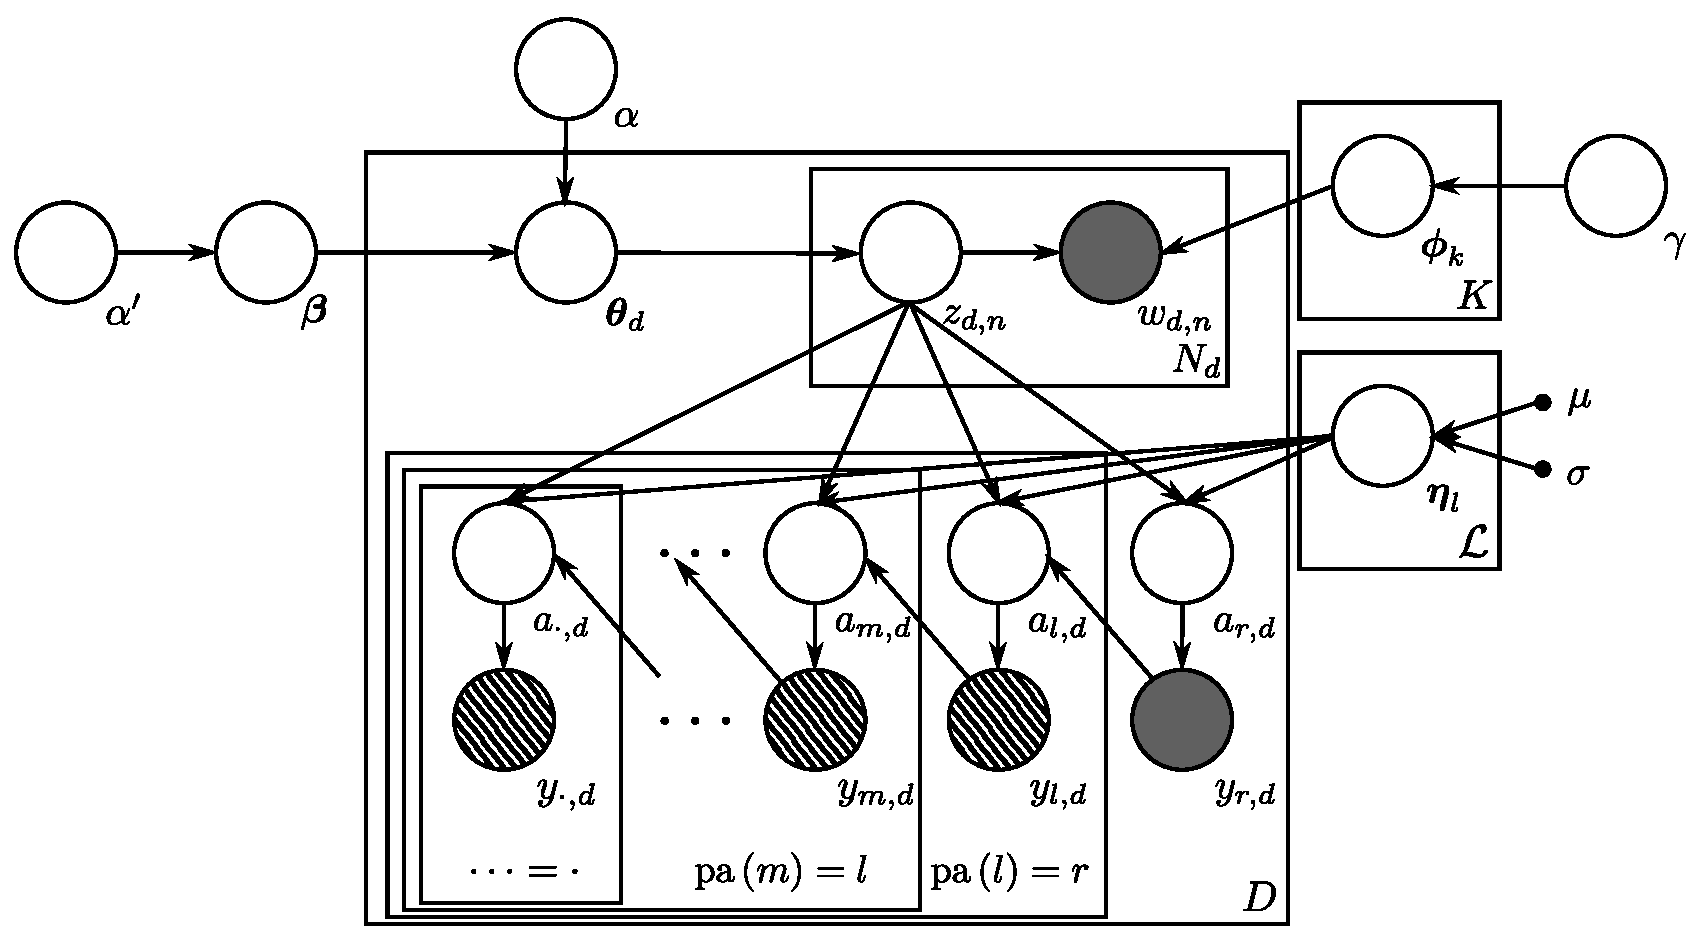
\includegraphics[scale=0.4]{Graphical_Model-final} \caption{adapted sLDA model}


\label{fig:example} 
\end{figure}


The fixed parameters of the model are the number of topics $K$, the
number of unique words in the vocabulary $V$, the number of documents
$D$, as well as the mean, $\boldsymbol\mu$, and the standard deviation, $\sigma$,
used in a normal prior distribution. The hyper-parameters $\alpha^{\prime}$,
$\alpha$, and $\gamma$ are weight parameters for Dirichlet prior
distributions. We will denote the $K$-dimensional Dirichlet distribution
as Dir$_{K}(\cdot)$ and the $K$ dimensional normal distribution
as $\mathcal{N}_{K}(\cdot)$.

We will now describe the stochastic generative process which defines
our model. The graphical model is show in Figure~\ref{fig:example}.
%Given the number of topics, K, and broad gamma priors on hyperparameters,
%the generative process is as follows: 

\begin{enumerate}
\item For each topic $k=1,\ldots,K$

\begin{itemize}
\item Draw a distribution over words $\boldsymbol\phi_{k}\sim{\rm Dir}_{V}(\gamma\mathbf{1}_V)$%,
%where $\mathbf{1}$ is a vector of ones of length $V$ 
\end{itemize}
\item For each label $l\in\mathcal{L}$

\begin{itemize}
\item Draw a regression coefficient $\boldsymbol\eta_{l}\mid\mu,\sigma\sim\mathcal{N}_{K}(\mu \mathbf{1}_K,\sigma \mathbf{I}_{K})$,
where $\mathbf{I}_{K}$ is the $K$ dimensional identity matrix 
\end{itemize}
\item Draw the global topic proportions $\boldsymbol\beta\mid\alpha'\sim{\rm Dir}_{K}\left(\alpha^{\prime}\mathbf{1}_K\right)$
\item For each document $d=1,\ldots,D$

\begin{itemize}
\item Draw topic proportions $\boldsymbol\theta_d\mid\boldsymbol\beta,\alpha\sim{\rm Dir}_{K}\left(\alpha\boldsymbol\beta\right)$ 
\item For $n=1,\ldots,N_{d}$

\begin{itemize}
\item Draw topic assignment $z_{n,d}\mid\boldsymbol\theta_d\sim{\rm Multinomial}(\boldsymbol\theta_d)$ 
\item Draw word $w_{n,d}\mid z_{n,d},\boldsymbol\beta_{1:K}\sim{\rm Multinomial}(\boldsymbol\beta_{z_{n,d}})$ 
\end{itemize}
\item For each label $l\in\mathcal{L}$: 

\begin{itemize}
\item Draw $a_{l,d}\mid \bar{\mathbf{z}}_d,\boldsymbol\beta_{l},y_{\mathrm{pa}(l),d}\sim\begin{cases}
\mathcal{N}(\bar{\mathbf{z}}^{T}\boldsymbol\eta_{l},1), & y_{\mathrm{pa}(l)}=1\\
\mathcal{N}(\bar{\mathbf{z}}^{T}\boldsymbol\eta_{l},1)\mathbb{I}(a_{l,d}<0), & y_{\mathrm{pa}(l)}=-1\end{cases}$ \\where $\bar{z}_{d}=N_{d}^{-1}\sum_{n=1}^{N}z_{n,d}$ %\item Draw $a_{l, d} \ | \ z_{1:N_d,d}, \boldsymbol\beta_l \sim \mathcal{N} \left(\bar z_d^{T} \boldsymbol\beta_{l},1\right)$, where $\bar z_d=N_d^{-1}\sum_{n=1}^{N_d}z_{n,d}$ 
 
\item Set the response variable \[
y_{l,d}\mid a_{l,d}=\begin{cases}
\ \ \ 1 & \text{if \ensuremath{a_{l,d}>0} and \ensuremath{y_{{\rm \mathrm{pa}}(l),d}=1}}\\
-1 & \text{otherwise}\end{cases}\]
 
\end{itemize}
\end{itemize}
\end{enumerate}
This type of generative model is known as a probit regression model.
Probit regression models are a type of discriminative probabilistic
model similar to logistic regression. However, instead of using the
logistic sigmoid as the link function, the probit regression model
uses the CDF for a standard normal distribution - the inverse of which
is known as the probit. In this case, the regression is conditional
on the parents according to the constraints of the labeling hierarchy.
The latent variables $a_{l,d}$ utilized here are also known as an
auxiliary variables because the are introduced to make exact Gibbs
sampling possible and are not of primary interest.

Given that negative labels are uncommon and that the absence of a
label is not equivalent to a negative label, we apply an informative
prior to the regression parameters, $\mathbf{\boldsymbol\beta}_{\mathcal{L}}$,
in the form of a negative prior that encodes a bias towards being
truly negative in the absence of a label.



\section{Inference}
\label{sec:inference}

\label{sec:inference}
Our inference goal  is to obtain a representation of the posterior distribution
of the latent variables in the model.  The posterior distribution we seek does not have a simple analytic form from which exact samples can be drawn.
This is usually the case for posterior distributions of non-trivial
probabilistic models and suggests a approximating the posterior distribution by sampling.

In this section we derive the conditional distributions required to sample from the HSLDA posterior distribution using Markov chain Monte Carlo. 

XXX  A very brief review of Markov chain Monte Carlo can be found in Section \ref{sec:mcmc} at the end of this chapter.  XXX

The HSLDA sampler, like the collapsed Gibbs samplers for LDA \cite{Griffiths04}, is itself a collapsed Gibbs sampler in which all of the latent variables that can be analytically marginalized are.  Among others, the parameters $\boldsymbol{\phi}_{1:K}$
and $\boldsymbol{\theta}_{1:D}$ are analytically marginalized prior to deriving the following conditional distributions for sampling.  
  It will often be the
case that the set of labels $\mathcal{L}$ is not fully observed for
every document. We will define $\mathcal{L}_{d}$ to be the subset
of labels which have been observed for document $d$. In an is-a hierarchical regression  it is straightforward
to marginalize the variables $a_{l^{\prime},d}$ and $y_{l^{\prime},d}$
for $l^{\prime}\in\mathcal{L}\backslash\mathcal{L}_{d}$ simply by ignoring them. 
%We can also integrate out the parameters $\boldsymbol{\phi}_{1:K}$
%and $\boldsymbol{\theta}_{1:D}$ as in \cite{Griffiths04}.
 The remaining latent variables (those that are not collapsed out) are $\mathbf{z}=\{z_{1:N_{d},d}\}_{d=1,\ldots,D},\boldsymbol\eta=\{\boldsymbol\eta_{l}\}_{l\in\mathcal{L}},\mathbf{a}=\{a_{l^{\prime},d}\}_{l^{\prime}\in\mathcal{L}_{d},d=1,\ldots,D},\boldsymbol\beta,\alpha,\alpha^{\prime}$
and $\gamma$.


%We will appeal to one of the common methods
%for approximating posterior distributions in the face of intractable
%normalization factors: Markov chain Monte Carlo (MCMC) sampling. 
%Since
% the conditional distributions
%for all variables are relatively simple (enumeration and, in the case of the profit regression coefficients, conjugate) we will use Gibbs sampling. %In particular, we will derive a collapsed Gibbs sampler.
%Given an observation of a set of observed labels and a document, the posterior distribution for the latent variables is
%\begin{equation}
%p\left(\theta,z_{1:N},\phi_{1:K},\boldsymbol\eta_{i_{l,c}\in\mathcal{I}},a_{i_{l,c}\in\mathcal{I}},\boldsymbol\beta,\alpha,\alpha',\gamma\mid w_{1:N},y_{i_{l,c}\in\mathcal{I}};\sigma,\lambda\right)\label{eq:Posterior}\end{equation}
%\[
%=\frac{p\left(\theta,z_{1:N},\phi_{1:K},\boldsymbol\eta_{i_{l,c}\in\mathcal{I}},a_{i_{l,c}\in\mathcal{I}},\boldsymbol\beta,\alpha,\alpha',\gamma,w_{1:N},y_{i_{l,c}\in\mathcal{I}};\sigma,\lambda\right)}{\int_{\theta,\phi,a,\boldsymbol\eta,\alpha,\alpha',\boldsymbol\beta,\gamma}\sum_{z}p\left(\theta,z_{1:N},\phi_{1:K},\boldsymbol\eta_{i_{l,c}\in\mathcal{I}},a_{i_{l,c}\in\mathcal{I}},\boldsymbol\beta,\alpha,\alpha',\gamma,w_{1:N},y_{i_{l,c}\in\mathcal{I}};\sigma,\lambda\right)}\]
%
%

\subsection{Gibbs Sampler}
 Let $\mathbf{a}$ be the set of all auxiliary variables, $\mathbf{w}$  the set of all words, $\boldsymbol\eta$  the set of all regression coefficients, and  $\mathbf{z}\backslash z_{n,d}$  the set $\mathbf{z}$ with element $z_{n,d}$ removed.  %The conditional posterior distribution of the latent topic indicators is
 %We use the notation $\mathbf{z}_{-(n,d)}$ to
%denote $\mathbf{z}_d\backslash z_{n,d}$. %, marginalizing
%$\theta_{1:D}$ and $\phi_{1:K}$. For details regarding collapsing
%in LDA models see \cite{Griffiths04}. 



%\subsection{Sampling latent topic indicators}
%$p(z_{n,d}\mid\mathbf{z}_{-(n,d)},\mathbf{a},\mathbf{w},\mathbf{\boldsymbol\eta},\alpha,\boldsymbol\beta,\gamma)$}

First we consider the conditional distribution of $z_{n,d}$ (the assignment variable
for each word $n=1,\ldots,N_{d}$ in documents $d=1,\ldots,D$). 
%The
%conditional distribution does not include $\theta_{1:D}$ and $\phi_{1:K}$
%because they have been integrated out as in the collapsed Gibbs sampler
%\cite{Griffiths04}. 
%The conditional distribution of $z_{n,d}$ is
%proportional to the joint distribution of its markov blanket. \begin{equation}
%p\left(z_{d,n}\mid\mathbf{z_{-\left(d,n\right)}},\mathbf{a},\mathbf{w},\mathbf{\boldsymbol\eta},\alpha,\boldsymbol\beta,\gamma\right)\propto p\left(z_{d,n},\mathbf{z_{-\left(d,n\right)}},\mathbf{a},\mathbf{w},\mathbf{\boldsymbol\eta},\alpha,\boldsymbol\beta,\gamma\right)\end{equation}
Following the factorization of the model (refer again to Figure~\ref{fig:graphical_model}), we can write
\begin{eqnarray*}
\lefteqn{p\left(z_{n,d}\mid\mathbf{z}_d\backslash z_{n,d},\mathbf{a},\mathbf{w},\mathbf{\boldsymbol\eta},\alpha,\boldsymbol\beta,\gamma\right)}\\
&\propto&\prod_{l\in\mathcal{L}_{d}}p\left(a_{l,d}\mid\mathbf{z},\boldsymbol\eta_{l}\right)p\left(z_{n,d}\ |\ \mathbf{z}_d\backslash z_{n,d},\mathbf{a},\mathbf{w},\alpha,\boldsymbol\beta,\gamma\right).\end{eqnarray*}
 The product is only over the subset of labels $\mathcal{L}_{d}$
which have been observed for document $d$. By isolating terms that
depend on $z_{n,d}$ and absorbing all other terms into a normalizing
constant as in \cite{Griffiths04} we find 
\begin{eqnarray}
\lefteqn{p\left(z_{n,d}=k\mid\mathbf{z}\backslash z_{n,d},\mathbf{a},\mathbf{w},\mathbf{\boldsymbol\eta},\alpha,\boldsymbol\beta,\gamma\right)\propto} \label{eq:z-likelihood} \\
 & \hspace{2cm}\left(c_{\left(\cdot\right),d}^{k,-\left(n,d\right)}+\alpha\boldsymbol\beta_{k}\right)\frac{c_{w_{n,d},\left(\cdot\right)}^{k,-\left(n,d\right)}+\gamma}{\left(c_{\left(\cdot\right),\left(\cdot\right)}^{k,-\left(n,d\right)}+V\gamma\right)}\prod_{l\in\mathcal{L}_{d}}\exp\left\{ -\frac{\left(\bar{\mathbf{z}}_{d}^{T}\boldsymbol\eta_{l}-a_{l,d}\right)^{2}}{2}\right\}\nonumber\end{eqnarray}
 where $c_{v,d}^{k,-\left(n,d\right)}$ is the number
of words of type $v$ in document $d$ assigned to topic $k$ omitting
the $n$th word of document $d$. The subscript $(\cdot)$'s
indicate to sum over the range of the replaced variable, i.e.~$ {c_{w_{n,d},\left(\cdot\right)}^{k,-\left(n,d\right)}} = \sum_d {c_{w_{n,d},d}^{k,-\left(n,d\right)}}$.  Here $\mathcal{L}_{d}$ is the set of labels which are observed for document $d$.  We sample from \eqref{eq:z-likelihood}  by enumeration and implicit normalization.
%
%Given Equation \ref{eq:z-likelihood}, $p\left(z_{d,n}\mid\mathbf{z}_{-\left(d,n\right)},\mathbf{a},\mathbf{w},\mathbf{\boldsymbol\eta},\alpha,\boldsymbol\beta,\gamma\right)$
%can be sampled through enumeration. 

The conditional posterior distribution of the regression coefficients is given by 
\begin{equation}
p(\boldsymbol\eta_{l}\mid\mathbf{z},\mathbf{a},\sigma) = \mathcal{N}(\hat{\boldsymbol\mu}_{l},\hat{\mathbf{\Sigma}})\label{eqn:regression_param_conditional}
\end{equation}
$\boldsymbol\eta_{l}$ for $l\in\mathcal{L}$. Given that $\boldsymbol\eta_{l}$
and $a_{l,d}$ are distributed normally, the posterior distribution
of $\boldsymbol\eta_{l}$ is normally distributed with mean $\hat{\boldsymbol\mu}_{l}$
and covariance $\hat{\mathbf{\Sigma}}.$% such that % (probably not the right place for this) We evaluated the model over various values of $\sigma$ where $\sigma=\left\{ 0.01,0.1,0.25,1,2\right\} $.
where
\begin{equation*}
\hat{\boldsymbol\mu}_{l}  =  \hat{\mathbf{\Sigma}}\left(\mathbf{1}\frac{\mu}{\sigma}+\bar{\mathbf{Z}}^{T}\mathbf{a}_{l}\right) \qquad \hat{\mathbf{\Sigma}}^{-1}  =  \mathbf{I}\sigma^{-1}+\bar{\mathbf{Z}}^{T}\bar{\mathbf{Z}}
.\end{equation*}
Here $\bar{\mathbf{Z}}$ is a $D\times K$ matrix
such that row $d$ of $\mathbf{\bar{Z}}$ is $\bar{\mathbf{z}}_{d}$, and $\mathbf{a}_{l}=[a_{l,1},a_{l,2},\ldots,a_{l,D}]^{T}$.  The simplicity of this conditional distribution follows from the choice of probit regression  \cite{Albert_Chib_1993}; the specific form of the update is a standard result from Bayesian normal  linear regression \cite{gelmanbda04}. 
%p\left(\boldsymbol\eta_{i_{l,c}}\mid\mathbf{z}_{1:D},\mathbf{a};\sigma\right)=\mathcal{N}\left(\boldsymbol\eta_{i_{l,c}}\mid\hat{\mu}_{i},\hat{\Sigma}_{i}\right)\end{equation}
%\[
%\[
%\subsection{$p\left(a_{l,d}\mid\mathbf{z},\mathbf{Y},\mathbf{\boldsymbol\eta}\right)$}
%and \textmd{$p\left(y_{m,i}\mid\mathbf{a}\right)$}}
%The auxiliary variables $a_{l,d}$ must be sampled for documents $d=1,\ldots,D$
%and $l\in\mathcal{L}_{d}$. The conditional posterior distribution
%of 
It also is a standard probit regression result that the conditional posterior
distribution of $a_{l,d}$ is a truncated normal
distribution~\cite{Albert_Chib_1993}. 
\begin{eqnarray*}
\lefteqn{p\left(a_{l,d}\mid\mathbf{z},\mathbf{Y},\mathbf{\boldsymbol\eta}\right)}\\&\propto&
\begin{cases}
\exp\left\{ -\frac{1}{2}\left(a_{l,d}-\boldsymbol\eta_{l}^{T}\mathbf{\bar{z}}_{d}\right)\right\} \mathbb{I}\left(a_{l,d}y_{l,d}>0\right)\mathbb{I}(a_{l,d}<0) , & y_{\mathrm{pa}(l),d}=-1\\
\exp\left\{ -\frac{1}{2}\left(a_{l,d}-\boldsymbol\eta_{l}^{T}\mathbf{\bar{z}}_{d}\right)\right\} \mathbb{I}\left(a_{l,d}y_{l,d}>0\right) , & y_{\mathrm{pa}(l),d}=1\end{cases}\label{eqn:a_l_d}\end{eqnarray*}

%\begin{equation}
%p\left(a_{l,d,}\mid\mathbf{z},\mathbf{Y},\mathbf{\boldsymbol\eta}\right)\propto\frac{1}{\sqrt{2\pi}}\exp\left\{ -\frac{1}{2}\left(a_{l,d}-\boldsymbol\eta_{l}^{T}\mathbf{\bar{z}}_{d}\right)\right\} \mathbb{I}\left(a_{l,d}y_{l,d}>0\right).\label{eqn:a_l_d}\end{equation}
% This conditional distribution can be sampled using an inverse CDF
%method. %However, if $y_{d,i_{l,c}}$ is unobserved then $a_{d,i_{l,c}}$must
%be sampled jointly with $y_{d,i_{l,c}}$ to ensure that the Markov
%chain is ergodic. Suppose that $a_{d,i_{l,c}}$ is sampled to have
%a negative value and $y_{d,i_{l,c}}$ is apporopriately sampled at
%-1. Although there exist valid states where $a_{d,i_{l,c}}>0$ and
%$y_{d,i_{l,c}}=1$, they will never be reached by such a Markov chain
%since $p\left(a_{d,i_{l,c}}<0\mid y_{d,i_{l,c}}=-1\right)=1$ and
%$p\left(y_{d,i_{l,c}}=-1\mid a_{d,i_{l,c}}<0\right)=1$. Therefore,
%to ensure ergodicity, $a_{d,i_{l,c}}$and $y_{d,i_{l,c}}$ must be
%sampled from the joint distribution as shown in Equation \ref{eq:Probit-Joint}.
%\begin{equation}
%p\left(a_{d,i_{l,c}},y_{d,i_{l,c}}\mid\mathbf{z},\mathbf{Y}_{-\left(d,i_{l,c}\right)},\mathbf{\boldsymbol\eta}\right)\propto p\left(y_{i_{l,c}}\mid\mathbf{a},\mathbf{y}_{-\left(l,c\right)}\right)p\left(a_{d,i_{l,c}}\mid\mathbf{z},\mathbf{Y},\mathbf{\boldsymbol\eta}\right)\end{equation}
%\begin{equation}
%p\left(y_{i_{l,c}}\mid\mathbf{a},\mathbf{y}_{-\left(l,c\right)}\right)=\delta\left(sign\left(a_{d,i_{l,c}}\right)=y_{i_{l,c}}\right)p\left(y_{i_{l,c}}\mid y_{parents_{l,c}}\right)\prod_{i_{\hat{l},\hat{c}}\in children_{l,c}}p\left(y_{i_{\hat{l},\hat{c}}}\mid y_{i_{l,c}}\right)\end{equation}
%\begin{equation}
%p\left(y_{i_{l,c}}=-1\mid y_{parent{}_{l,c}}\right)=\begin{cases}
%1, & y_{parent_{l,c}}=-1\\
%0.5, & y_{parent_{l,c}}=1\end{cases}\end{equation}
%\[
%p\left(a_{d,i_{l,c}},y_{d,i_{l,c}}\mid\mathbf{z},\mathbf{Y}_{-\left(d,i_{l,c}\right)},\mathbf{\boldsymbol\eta}\right)\]
%\begin{equation}
%=\begin{cases}
%\mathcal{N}\left(a_{d,i_{l,c}}\mid\bar{z}^{T}\boldsymbol\eta_{i_{l,c}},1\right)p\left(y_{d,i_{l,c}}\mid a_{d,i_{l,c}}\right), & y_{parent_{l,c}}=1,\forall y_{i_{\hat{l},\hat{c}}}\in y_{children_{l,c}},y_{i_{\hat{l},\hat{c}}}=-1\\
%trunc\mathcal{N}^{-}\left(a_{d,i_{l,c}}\mid\bar{z}^{T}\boldsymbol\eta_{i_{l,c}},1\right)\delta\left(y_{d,i_{l,c}}=-1\right), & y_{parent_{l,c}}=-1\\
%trunc\mathcal{N}^{+}\left(a_{d,i_{l,c}}\mid\bar{z}^{T}\boldsymbol\eta_{i_{l,c}},1\right)\delta\left(y_{d,i_{l,c}}=1\right), & \exists y_{i_{\hat{l},\hat{c}}}\in y_{children_{l,c}}\setminus y_{i_{\hat{l},\hat{c}}}=1\\
%0 & otherwise\end{cases}\end{equation}
%where $\mathbf{Y}_{-\left(d,i_{l,c}\right)}$ denotes all of the response
%variables excluding the response variable being sampled.
%
%
%
%\subsection{$p\left(\boldsymbol\beta\mid\mathbf{z},\alpha^{\prime},\alpha\right)$}

%Note that care must be taken to initialize the Gibbs sampler in a valid state.

HSLDA employs a hierarchical Dirichlet prior over topic assignments (i.e.,~$\boldsymbol\beta$ is estimated from data rather than fixed a priori).  This has been shown to improve the quality and stability of inferred topics \cite{WallachMiMc2009}. 
%This prior
%shares many features with the hierarchical Dirichlet process and inference
%over this distribution proceeds in a very similar fashion.
%
Sampling $\boldsymbol\beta$, the vector of global topic proportions,   can be done using the ``direct assignment''
method of \cite{TehJorBea2006} \begin{equation}
\boldsymbol\beta\mid\mathbf{z},\alpha^{\prime},\alpha\sim{\rm Dir}\left(m_{\left(\cdot\right),1}+\alpha^{\prime},m_{\left(\cdot\right),2}+\alpha^{\prime},\ldots,m_{\left(\cdot\right),K}+\alpha^{\prime}.\right)\end{equation}
Here $m_{d,k}$ are auxiliary variables that are required to sample the posterior distribution of $\boldsymbol\beta$.  Their conditional posterior distribution is sampled according to
 \begin{equation}
p\left(m_{d,k}=m\mid\mathbf{z},\mathbf{m}_{-\left(d,k\right)},\boldsymbol\beta\right)=\frac{\Gamma\left(\alpha\boldsymbol\beta_{k}\right)}{\Gamma\left(\alpha\boldsymbol\beta_{k}+c^k_{(\cdot),d}\right)}s\left(c^k_{(\cdot),d},m\right)\left(\alpha\boldsymbol\beta_{k}\right)^{m}\end{equation}
where $s\left(n,m\right)$ represents stirling numbers of the first
kind.


%\subsection{$p\left(\alpha\right)$, $p\left(\alpha'\right)$, $p\left(\gamma\right)$}

The hyperparameters $\alpha$, $\alpha^{\prime}$, and $\gamma$ are
%given broad ${\rm Gamma}(1,1000)$ prior distributions and 
sampled
using Metropolis-Hastings. 



\section{Related Work}

\label{sec:related_work} 
This chapter covers classifying or, equivalently, labeling bag-of-words data.  We show how to construct classifiers based on features derived from mixed membership models.  We specifically develop a solution to the concrete problem of hierarchically classifying text documents.  The model and techniques developed in this chapter can be used to solve any labeling or hierarchical classification problem involving data represented as bags-of-words.  For instance,  if an image is represented by counts of features then it can be described as being in a bag-of-words representation.   So, hierarchical classification of images might be tackled using the techniques developed in this chapter, although, such a particular application will not be explicitly considered.

We should agree that classification and regression are largely the same.  Namely, classification is regression with discrete output.  To solve classification problems we must learn from training instances, as in regression, a function $f : \mathcal{X} \rightarrow \mathcal{L}$ which maps from an input space $\mathcal{X}$ to an output (label) space $\mathcal{L}$.   For example, consider the problem of identifying the authors of a set of documents for which the true author is unknown but is one of a set of possible authors.   For such a problem the input space is the richly structured space of possible texts and the output space is the large but largely unstructured list of possible authors.  Training data would consist of text author pairs for texts known to have been authored by authors in the list of possible authors.

To solve such a problem one would need to choose a set of features to extract from the underlying documents. Then, using those features and the training data, a classification function would be learned.  In this case one might choose a multi-class logistic or probit regression function and learn parameters for it from the labeled training instances.   In this chapter we will focus on models that use mixed-membership representations of bag-of-word data as the input features to joint models that can be used, via conditioning, for classification or regression.

The models that we propose in this chapter generalize the author classification example in that the label spaces we will consider are also richly structured (in addition to the input space) and the regression function we learn maps from from the input space to labels in a structured, typically hierarchical label space.  In the same way that mixed membership models are surprisingly effective, the resulting hierarchical classification models seem to be too.

\subsection{Background}

Mixed membership models, particularly latent Dirichlet allocation (LDA) \cite{Blei2003}, have been reviewed in other chapters.   The key property we exploit for purposes of classification is that LDA % is a generative
%probabilistic model of corpora consisting of documents that are bag-of-words.  In particular LDA 
provides a way to extract a latent, low-dimensional representation of each bag-of-words observation consisting of mixing proportions over topic vectors.  Each topic is a frequency histogram of terms.  Each document is a mixture of topics.  This mixture of topics vector is the feature vector we exploit for purposes of document classification.  

%Also known as topic models, these models
%infer the latent structure, or topics, of documents in a corpus. Each
%document is represented as a collection of words, generated from a
%set of topic assignments (one for each word), where each topic assignment
%is drawn from a distribution over topics \cite{Blei2003}.

The idea for using this representation for classification was first considered in a paper on so-calling ``supervised'' latent Dirichlet allocation (SLDA).  SLDA built on LDA by incorporating
``supervision'' in the form of an observed exponential family response 
variable per document.  Another way of saying this is that SLDA was the first document classifier for documents in the bag-of-words representation that exploited the LDA topic feature representation.  
%A subtle point should be noted here. 
 SLDA and the subject of this chapter, a generalization of it called hierarchically supervised LDA (HSLDA) \cite{Perotte-2012-NIPS} are not, strictly speaking, regression models.  This is because they model the {\em joint} distribution of labels and bag-of-words data rather than the conditional distribution of the labels given the input.   Having the joint distribution allows us to condition on an input to produce a label for all test instances.  Additionally, during training of the model, knowing the labels effects the learning of the low dimensional representation of the input -- a characteristic discussed later in this chapter.
% This is quite different (and better performing in practice) than LASSO
%(L1 regularized least squares regression) and LDA followed by least
%squares regression \cite{BleiMcAuliffe2008}.
%By performing joint inference, SLDA and HSLDA
%infer topics such that the model predicts the response variable while
%improving word likelihood.  

%In this chapter we extend supervised latent Dirichlet allocation (SLDA)
%\cite{BleiMcAuliffe2008} to take advantage of hierarchical supervision. SLDA
%is latent Dirichlet allocation (LDA) \cite{Blei2003} augmented with per
%document ``supervision,'' often taking the form of a single numerical or
%categorical label. It has been demonstrated that the signal provided by such
%supervision can result in better, task-specific document models and can also
%lead to good label prediction for out-of-sample data \cite{BleiMcAuliffe2008}.

%It also has been demonstrated that SLDA has been shown to outperform both LASSO
%(L1 regularized least squares regression) and LDA followed by least squares
%regression~\cite{BleiMcAuliffe2008}. 

The problem of applying structured labels to bag-of-words data can be tackled in a number of different ways.  For instance,  SLDA can be used to solve this kind of problem directly; however, doing so requires ignoring the hierarchical
dependencies amongst the labels. In Section~\ref{sec:experiments} we contrast
HSLDA with SLDA applied in this way. 
Other models that incorporate LDA and supervision and so could be used to solve this problem include
LabeledLDA~\cite{Ramage2009} and DiscLDA~\cite{DiscLDA}.  Various applications of these models to 
computer vision and document networks have been explored~\cite{wangbleifeifei08,RelationalLDA}.
None of these models, however, leverage dependency structure in the label space.
%While there has been much work in multi-label classification of text and
%text modeling in general, we focus here on topic modeling approaches.
%Latent Dirichlet allocation (LDA) is a generative probabilistic model which
%represents documents as a mixed-membership bag of word. Each document is
%represented as a collection of words, generated from a set of topic assignments
%(one for each word), where each topic assignment is drawn from a distribution
%over topics~\cite{Blei2003}. SLDA is latent Dirichlet allocation (LDA)
%\cite{Blei2003} augmented with per-document labeling, often taking the form of
%a single numerical or categorical label. Examples of labels include ratings
%associated with online reviews, grades for essays, and the number of times a
%webpage is linked. This approach has been shown to outperform both LASSO
%(L1 regularized least squares regression) and LDA followed by least
%squares regression~\cite{BleiMcAuliffe2008}.





In other non-LDA-based related work, researchers have classified documents into a hierarchy (a closely related task) using naive Bayes classifiers
and support vector machines. Most of this work has been demonstrated on relatively
small datasets, small label spaces, and has focused on single label classification without
a model of documents such as LDA~\cite{mccallum99building,Dumais2000HCW,Kollerilprints291,Chakrabarti1998SFS}.  The HSLDA model we cover here is not limited in this way.

%One set of models that are particularly relevant to HSLDA are Chang
%and Blei's hierarchical models for document networks (Relational Topic
%Models). In that family of models, they encountered a similar scenario
%where the lack of a link did not truly indicate absence. In hierarchically
%labeled data, negative labels are uncommon and the lack of a label
%in the hierarchy is not equivalent to a negative label. Therefore,
%as in the work of Chang and Blei, we employ regularization to account
%for the lack of negative labels. This will be discussed further in

% Noemie: check out what I wrote here, because I am not really sure this is
% correct. 
%There have been several models that incorporate both latent models of text and
%some form of
%supervision~\cite{Ramage2009,DiscLDA,wangbleifeifei08,RelationalLDA}. One set 
%of models that are particularly relevant to HSLDA are Chang and Blei's
%hierarchical models for document networks (Relational Topic Models). In that
%family of models, they encountered a similar scenario where an unselected label 
%does not always indicate absence. In hierarchical labels, this phenomenon is
%even more pervasive -- there are no explicit negative labels, but it is also
%unclear how to treat the parents of selected labels. Like in the work of Chang
%and Blei, we employ regularization to account for the lack of negative
%labeling. In our experiments, we look at the impact of assigning positive and
%negative instances to the ancestors of selected labels.


\section{Experiments}

\label{sec:experiments}

%\begin{itemize}
%\item Describe Data for both Experiments
%\item Describe the Four different conditions
%\item Describe how they are all evaluated, with and without hierarchy
%\end{itemize}
In the section we describe the application of HSLDA for prediction
in two hierarchically structured domains. Firstly, we describe using
discharge summaries to predict diagnoses, encoded as ICD-9 codes.
Discharge summaries are documents that are authored by clinicians
to summarize the course of a hospitalization. ICD-9 codes are used
mainly for billing purposes to indicate the conditions for which a
patient was treated. Secondly, we describe using Amazon.com product
descriptions to predict product categories.


\subsection{Data and Pre-Processing}


\subsubsection{Diagnosis Prediction}

Our data set was gathered from the clinical data warehouse of NewYork-Presbyterian
Hospital. The data consisted of free-text discharge summaries and
their respective ICD-9 codes. A discharge summary is a clinical report
prepared by a physician or other health professional at the conclusion
of a hospital stay or series of treatments. The note outlines the
patient's chief complaint, diagnostic findings, therapy administered,
patient's response to the chosen therapy, the treatment plan and the
recommendations upon discharge. The ICD-9 codes used to structure
the discharge summary data are part of a controlled terminology which
is the international standard diagnostic classification for epidemiological,
health management, and clinical purposes. The ICD-9 codes are organized
in a rooted-tree structure, with each edge representing an is-a relationship
between parent and child, such that the parent diagnosis subsumes
the child diagnosis. For example, the code representing {}``Pneumonia
due to adenovirus'' is a child of the code representing {}``Viral
pneumonia'' where the former is a type of the latter. In the hospital,
ICD-9 codes are generated manually by trained medical coders, who
review all the information in the discharge summary.

The text of the discharge summaries were pre-processed such that each
document would be represented as counts over a 10,000 word vocabulary.
The Natural Language Toolkit was used to tokenize the text. A vocabulary
was identified by first sorting terms based on a global term frequency-inverse
document frequency measure. The top 10,000 words which were not identifying
in some way (a name, place, or identifying number) were selected for
inclusion in the vocabulary.

For each hospitalization there are usually several ICD-9 codes assigned
for billing purposes. These codes are known to be quite specific but
not very sensitive \citep{Birmetal2005}. Regardless of that fact,
this is one of the only sources for information on patient diagnoses
aside from the free text. %Aside from prediction, one of the goals is to compare the sensitivity of predictions from the HSLDA model in comparison to the codes in a case where a test closer to ground truth is available. For this we will compare whether predictions for the ICD-9 code associated with anemia are better predicted by HSLDA or by the ICD-9 codes. Anemia was chosen because hemoglobin values are readily available and the definition of anemia according the World Health Organization is approximately 12.5, with a threshold of 12 for women and 13 for men [citation].


We worked within the guidelines of the Health Insurance Portability
and Accountability Act (HIPAA), which protects patient privacy and
the security of potentially identifying medical material, known as
personal health information (PHI). HIPAA covers any information within
a medical record that was created, used, or disclosed during the course
of providing a health care service and that can be used to identify
an individual. This study was approved by the Institutional Review
Board.


\subsubsection{Product Category Prediction}

Data for these experiments were obtained partially from the Stanford
Network Analysis Platform (SNAP) Amazon product metadata dataset \citep{SNAP}
and partially directly from the the Amazon.com website \citep{AMAZON}.
The product ID's and categorizations were obtained from the SNAP dataset
and the product descriptions were obtained directly from the website.

We were able to deduce the structure of the hierarchy for the Amazon.com
products directly since all ancestors in the hierarchy were included
with each category label. For example, {}``DVD / Genres / Science
Fiction \& Fantasy / Classic Sci-Fi'' is a single product category
for the DVD, {}``The Time Machine''. Each product was labeled with
multiple categories.

The vocabulary for this experiment was created by including the most
frequent 30K words omitting stopwords.


\subsection{Comparison Models}

We applied HSLDA, along with three other closely related models, to
the clinical data and the retail product data. Specifically, we evaluate
models including sLDA with independent regressors (hierarchical constraints
on labels ignored), HSLDA fit by performing LDA followed by tree-conditional
regressions, and HSLDA fit with fixed random regression parameters.
We will refer to the three comparison models as the sLDA model, the
separate HSLDA model, and the random HSLDA model, respectively. These
models were chosen as to highlight performance in absence of hierarchical
constraints, the effect of the combined inference procedure, and regression
performance attributable solely to the hierarchical constraints.

We evaluated model performance for all three models with a range of
values for $\mu$ ($\mu\in\left\{ -3,-2.8,-2.6,\ldots,1\right\} )$,
the mean prior parameter for regression parameters.


\subsection{Evaluation}

%\begin{itemize}
%\item Talk about hierarchy and no hierarchy
%\item Make explicit calculation of sensitivity and 1-specificity
%\end{itemize}
For each dataset, a held out set of 1,000 documents and accompanying
labels were used for evaluation. The two main methods of evaluation
for the model are prediction and topic quality. To evaluate predictive
performance for all comparison models equivalently, each model was
evaluated with two methods. The first evaluation method augments the
observed labels in the held out set with their ancestors and considers
all other non-existant labels to be negative. The second method ignores
the ancestors of the observed labels in the held out set and considers
all other non-existant labels to be negative. This uniform treatment
of ancestors allows for a fair comparison of the models.

The two measures for predictive performance used here include the
true positive rate and the false positive rate evaluated based on
$p\left(y_{l,\hat{d}}\mid w_{1:N,d}\right)$ for each label in each
model.

\section{Results}
\label{sec:results}

\begin{figure}[htbp]
\begin{center}
\subfigure[][\label{1a}]{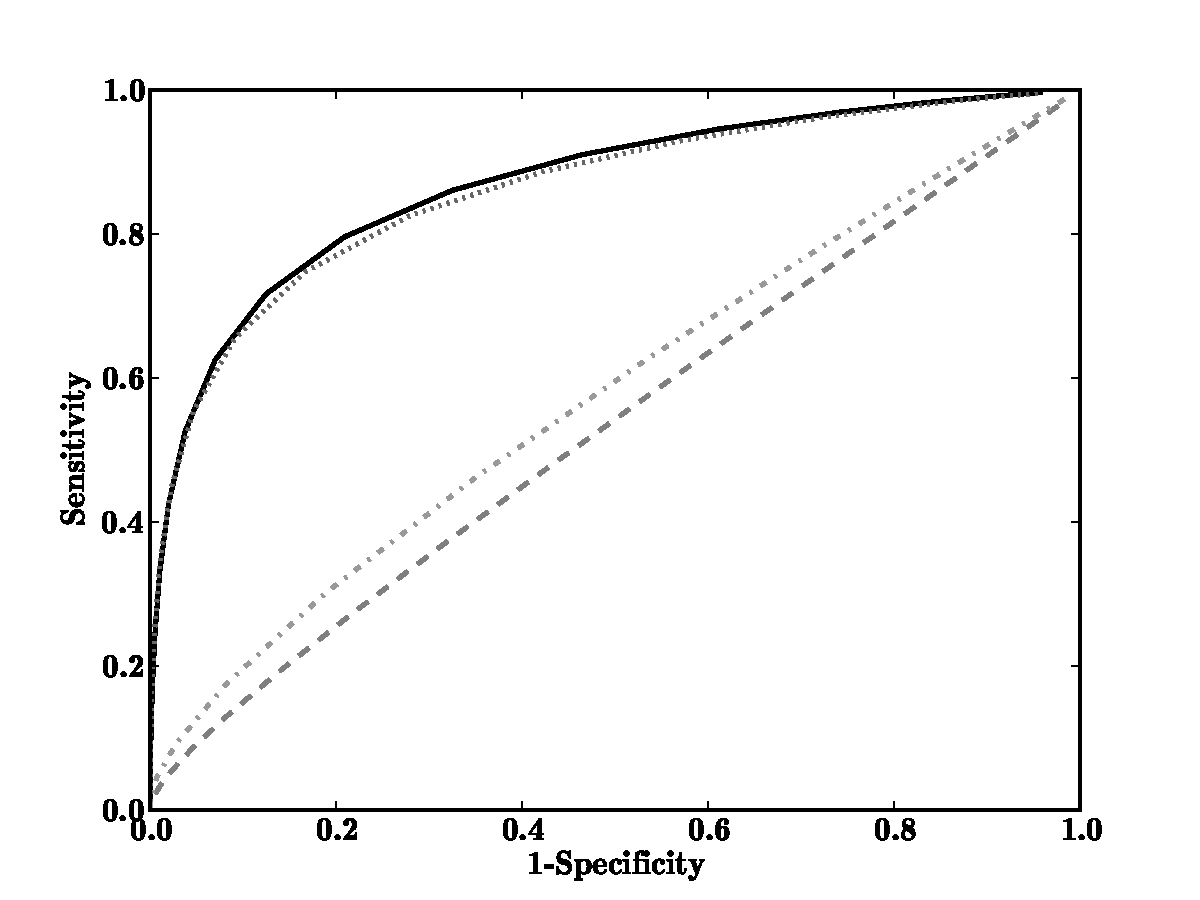
\includegraphics[width=.49\textwidth]{figs/ROC_comparison_ancestors}}
\subfigure[][\label{1b}]{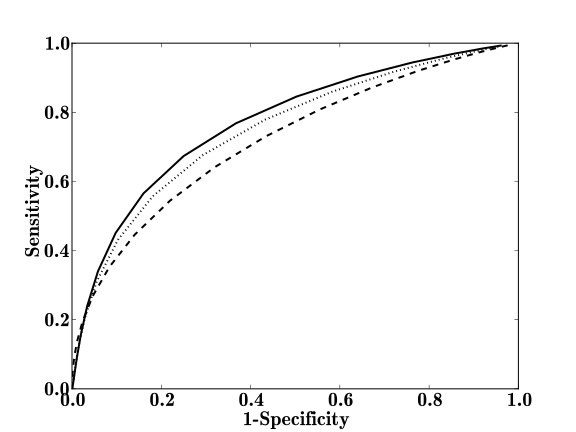
\includegraphics[width=.49\textwidth]{figs/ROC_comparison_leafs}}
\subfigure[][\label{1c}]{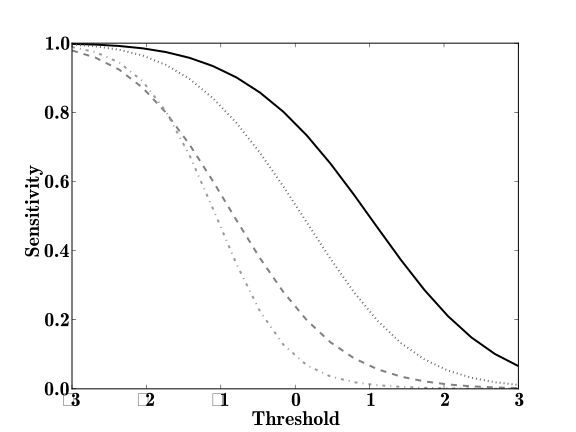
\includegraphics[width=.49\textwidth]{figs/sens_comparison_leafs}}
\subfigure[][\label{1d}]{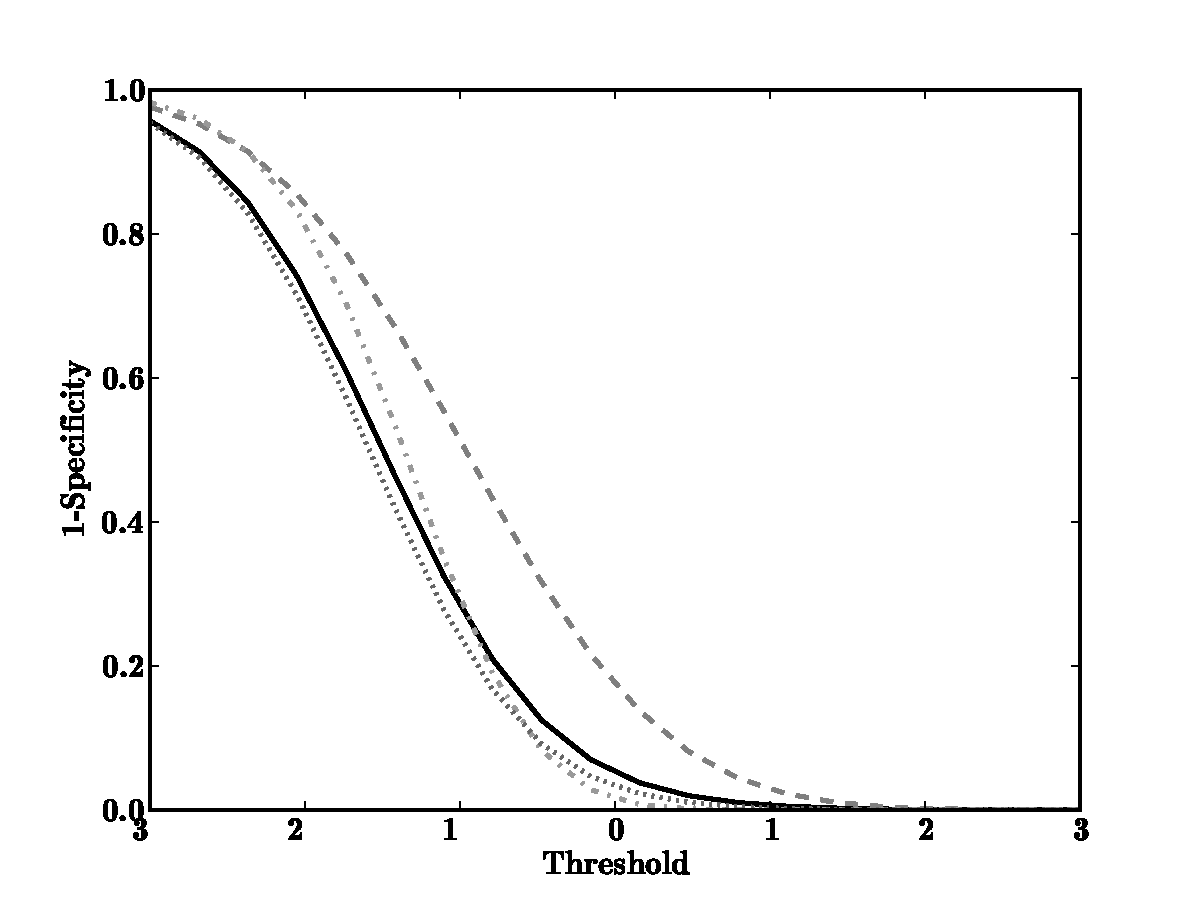
\includegraphics[width=.49\textwidth]{figs/one_m_spec_comparison_leafs}}
\caption{Out-of-sample ICD-9 code prediction from patient free-text discharge records.  In all figures solid is HSLDA, dashed are independent regressors + sLDA (hierarchical constraints on labels ignored), dotted is HSLDA fit by running LDA first then running tree-conditional regressions, and dot-dashed is HSLDA fit with fixed random regression parameters.  Top row:  \subref{1a} includes ancestor prediction performance,  \subref{1b} results are for given (leaf) labels alone.  Bottom row: \subref{1c} are the sensitivity curves from \subref{1b} aligned on threshold value,  \subref{1d} are the 1-specificity curves from \subref{1b} aligned on threshold value.}
\label{fig:icd9}
\end{center}
\end{figure}

\begin{figure}[htbp]
\begin{center}
\subfigure[][\label{2a}]{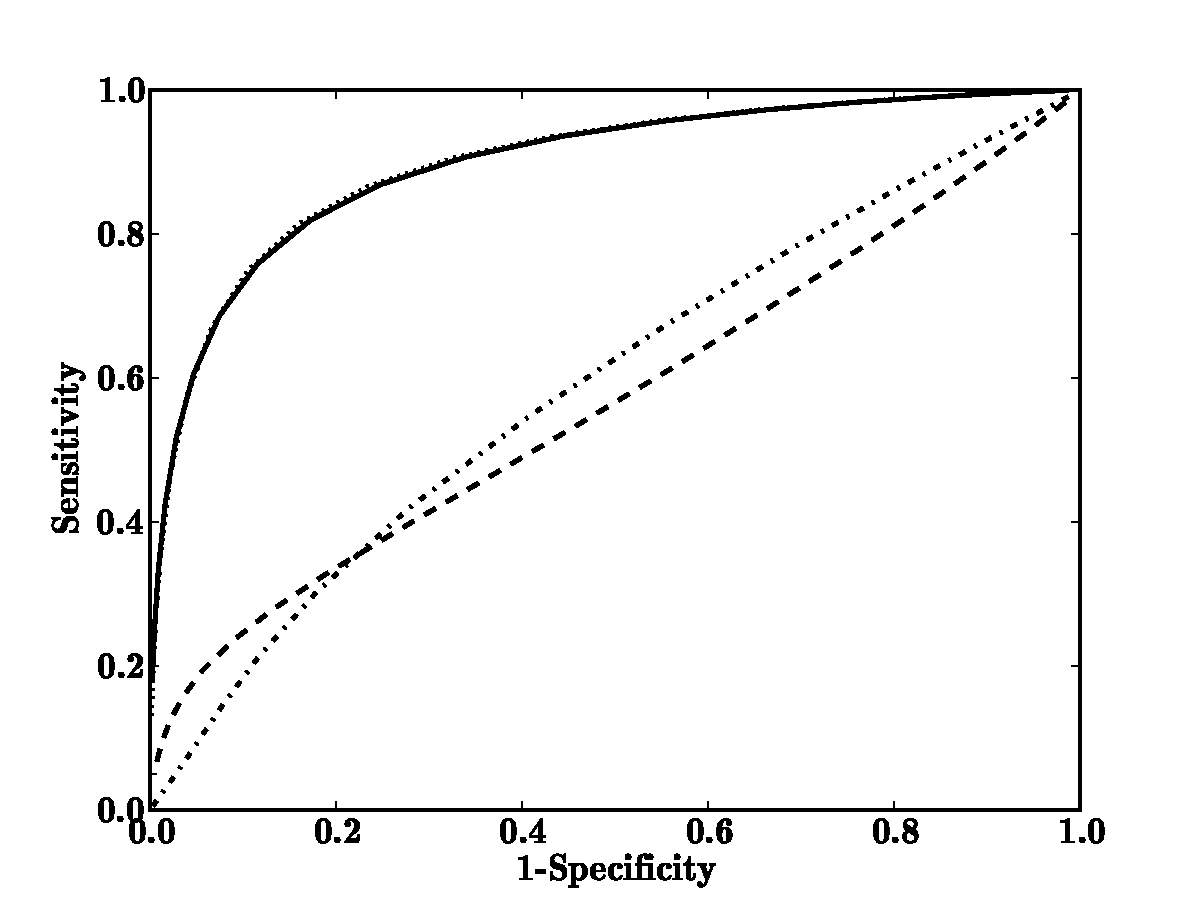
\includegraphics[width=.49\textwidth]{figs/ROC_comparison_ancestors_amazon}}
\subfigure[][\label{2b}]{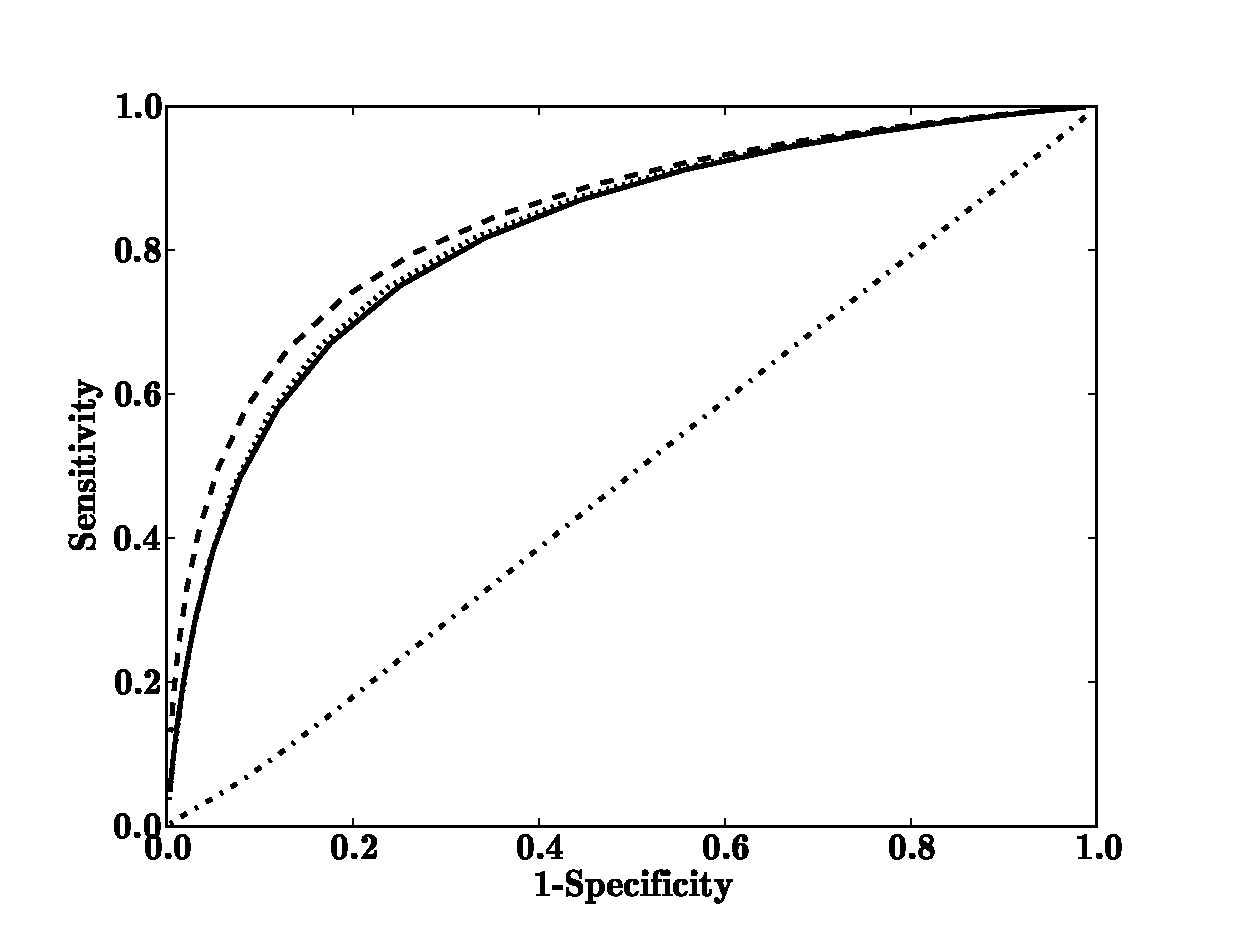
\includegraphics[width=.49\textwidth]{figs/ROC_comparison_leafs_amazon}}
\subfigure[][\label{2c}]{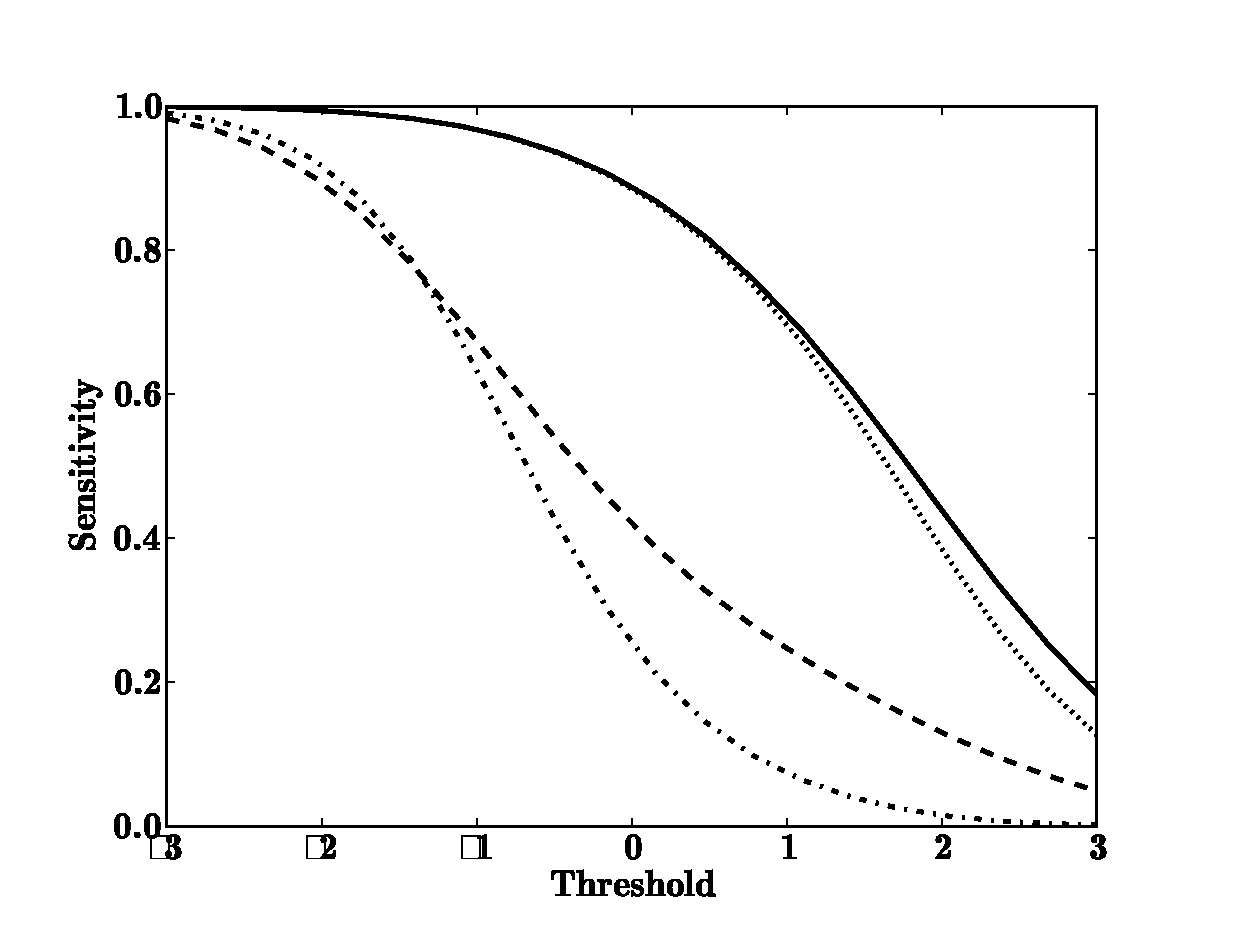
\includegraphics[width=.49\textwidth]{figs/sens_comparison_leafs_amazon}}
\subfigure[][\label{2d}]{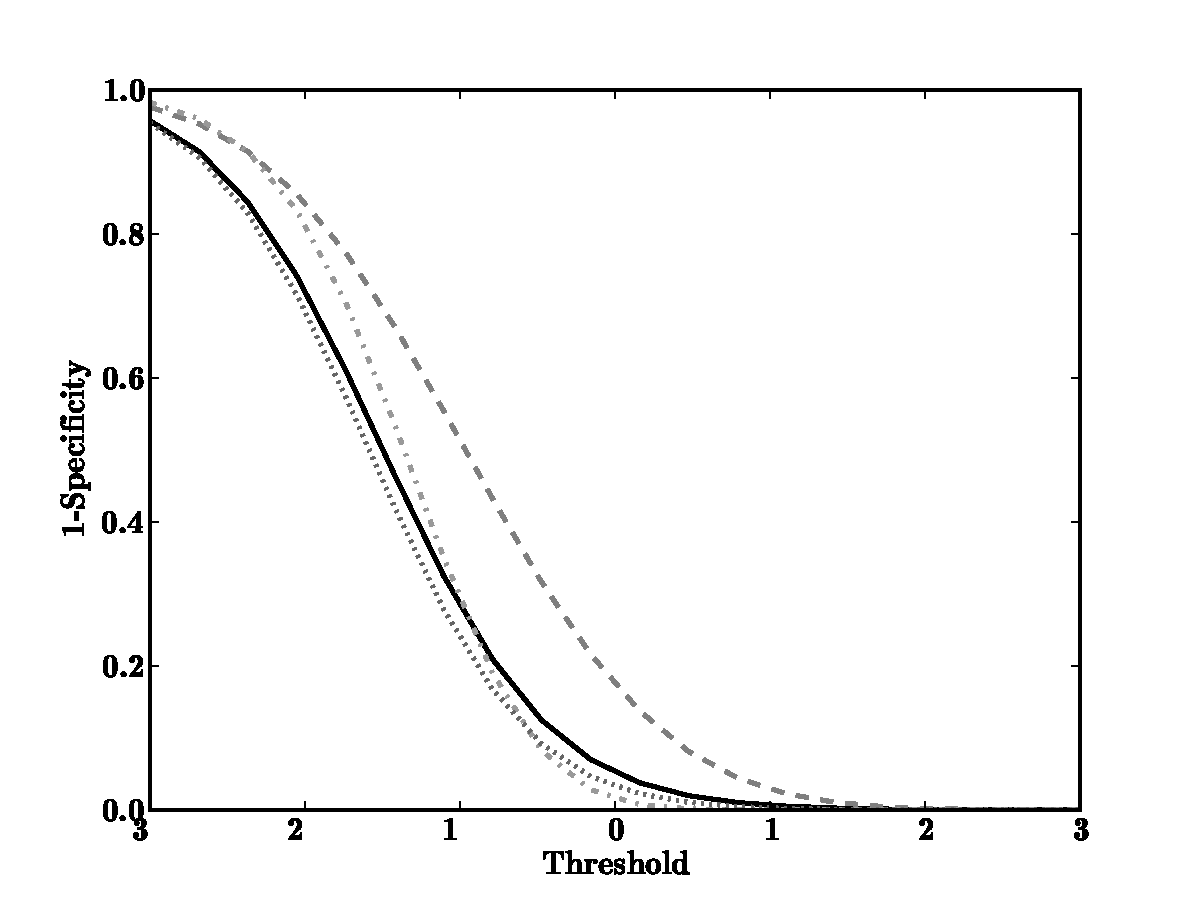
\includegraphics[width=.49\textwidth]{figs/one_m_spec_comparison_leafs}}
\caption{Out-of-sample Amazon product code predictions from product free-text descriptions.  In all figures solid is HSLDA, dashed are independent regressors + sLDA (hierarchical constraints on labels ignored), dotted is HSLDA fit by running LDA first then running tree-conditional regressions, and dot-dashed is HSLDA fit with fixed random regression parameters.  Top row:  \subref{2a} includes ancestor prediction performance,  \subref{2b} results are for given (leaf) labels alone.  Bottom row: \subref{2c} are the sensitivity curves from \subref{2b} aligned on threshold value,  \subref{2d} are the 1-specificity curves from \subref{2b} aligned on threshold value.}
\label{fig:icd9}
\end{center}
\end{figure}

%We ran the Gibbs sampler for two days on 500 documents with 20 topics to learn the sLDA model which we then followed by a prediction of ICD-9 codes for 100 documents. The prediction resulted in 38 documents with at least 1 ICD-9 code assignment while some had over 200 assignments.


%\begin{figure}[h]%tbp] %  figure placement: here, top, bottom, or page
%   \centering
%   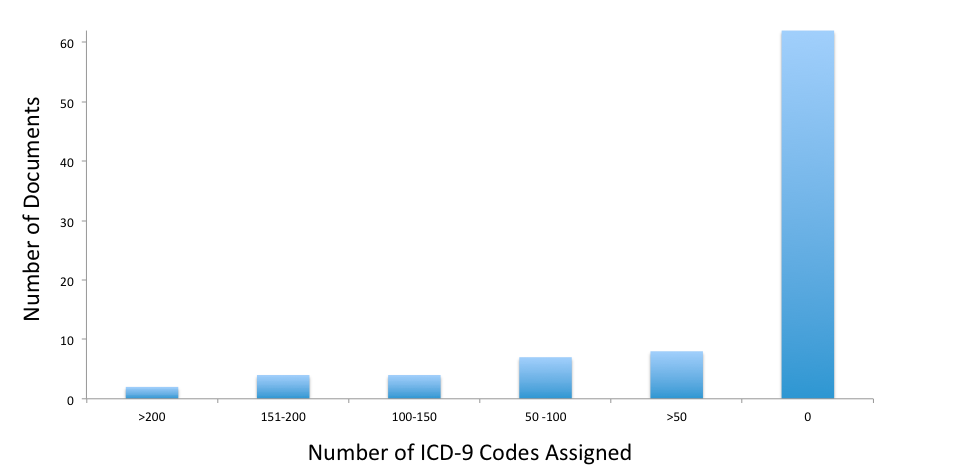
\includegraphics[width=4in]{number_of_codes_histogram} 
%   \caption{distribution of ICD-9 code assignments over all of the 100 documents predicted}
%   \label{fig:example}
%\end{figure}


%The accuracy of the prediction was tested against the actual ICD-9 codes in the EHR record for each discharge summary.  Different statistical measures were applied to asses the predictions.


%\begin{figure}[h]%tbp] %  figure placement: here, top, bottom, or page
%   \centering
%   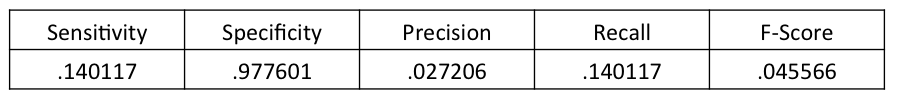
\includegraphics[width=4in]{signal_detection} 
%   \caption{sensitivity, specificity, precision, recall and F-measure.}
%   \label{fig:example}
%\end{figure}


%Although the sensitivty is not as high as we would have hoped, it is important to note that the sLDA was run on a very limited sample of documents (500) due to time constraints.  Additionally, the “gold standard” data used are actual hospital results which are very noisy given the incompleteness and introduction of human error.



\section{Discussion}
\label{sec:discussion}
%Despite the proliferation of LDA related models in recent years, one could argue that the true killer app for LDA has yet to be discovered.  LDA makes sense for information retrieval (IR) because  the learned latent topic vectors serve as good low-dimensional document representations, and, a posteriori similarity between such vectors can be used to compute the similarity of documents.  Unfortunately, computational considerations render this approach to IR impractical in most settings.

The SLDA model family, of which HSLDA is a member, can be understood in two different ways.  One way is to see it as a family of topic models that improve on the topic modeling performance of LDA via the inclusion of observed supervision.  Another way to see the family is as a set of models that can predict labels for bag-of-words data.  A large diversity of problems can be expressed as label prediction problems for bag-of-words data.  A surprisingly large amount of that kind of data possess structured labels, either hierarchically constrained or otherwise.  That HSLDA directly addresses this kind of data is a large part of the motivation for this work.   That it outperforms more straightforward approaches should be of interest to practitioners.

Variational Bayes has been the predominant estimation approach applied to sLDA models.  Hierarchical probit regression makes for tractable Markov chain Monte Carlo SLDA inference, a benefit that should extend to other sLDA models should probit regression be used for response variable prediction there too.  

The results in Figures~\ref{fig:1a} and \ref{fig:1b} suggest that in most cases it is better to do full joint estimation of HSLDA.  In alternative interpretation of the same results is that if one is more sensitive to the performance gains that result from exploiting the structure of the labels then one can, in an engineering sense, get nearly as much gain in label prediction performance by first fitting LDA and then fitting a hierarchical probit regression.  There are applied settings in which this could be advantageous.

Extensions to this work include unbounded topic cardinality variants and relaxations to different kinds of label structure.  Unbounded topic cardinality variants pose interesting inference challenges.  Utilizing different kinds of label structure is possible within this framework, but requires relaxing some of the simplifications we made in this paper for expositional purposes. 

%We have described a mixed membership model with hierarchical supervision. We have demonstrated this model in the context of document modeling with hierarchical multi-label supervision. Such a model is appropriate in domains where there are hierarchical constraints among the labels such as is the case in an IS-A hierarchy.

...

%\begin{itemize}
%\item what about the nonparametric version of this?
%\item discuss the broader goal, from the beginning of search engine time, to combine categorization and free text.  this, to our knowledge, is the first principled approach to doing so
%\end{itemize}

%We have proposed a new method for prediction of ICD-9 codes given a medical discharge summary note.  Our method explicitly takes advantage of the ICD-9 hierarchical IS-A relationships as well as the word distributions in each document.  We used Gibbs sampling for a supervised latent dirichlet allocation model to learn a distribution of words over twenty topics and their appropriate ICD-9 codes (response variable). The model was then tested on 100 discharge summaries for which the ICD-9 diagnoses were known.  The amount of ICD-9 codes produced for some discharge summaries was quite high because of the way the model worked with the IS-A hierarchy, highlighting the completeness of ICD-9 coding when using this sLDA model.  Overall, the model had extremely good specificity while the sensitivity was lower than anticipated.  Given our limited set of documents, and very noisy gold standard it would not be accurate to discount the use of sLDA in medical document classification and automatic coding.
%In future work, we plan to significantly expand the set of documents used to train the model (up to 15,000), as well as run several different iterations to learn the optimal topic number.  


%A more automated approach for coding patient visits with the ICD-9 hierarchy has great promise to  reduce health care costs and increase completeness of medical coded data.  We hope that this implementation of supervised LDA will serve as preliminary work for a much larger study with more documents in the future.


\begin{small} \bibliographystyle{plainnat} \bibliographystyle{plainnat}
\bibliographystyle{plainnat}
\bibliography{refs}


\end{small} 

\end{document}

